\section{INTRODUCTION}\label{sec:1introduction}

Sleep plays a vital role in good health and well-being throughout a person's life. Lacking of sleep or having poor sleep can lead to
serious, sometimes life-threatening, health problems~\cite{altena2008sleep,chandola2010effect,lallukka2016contribution}. The quality of
sleep depends on many factors, including the sleeping environment such as the light intensity and the ambient temperature, the user's
breath, the sleeping posture, and the bedtime routine. By capturing and modeling these factors, sleep monitoring can help users to assess
and understand their sleeping pattern, and provide feedback on how the change of the sleeping environment and behavior affect the sleep
quality.

Traditionally, sleep monitoring had to be performed in a clinic environment using dedicated medical equipment.  Modern mobile devices such
as smartphones and wearable devices offer a new way for sleep monitoring. By utilizing the rich mobile sensors, we can track certain
activities such as body movements or snore, and to use the tracked information to detect and model sleep
patterns~\cite{zeo,Jawbone,SleepAndroid,fitbit,gu2016sleep}. Such an approach is known as
\emph{actigraphy}~\cite{Actigraphy,ancoli2003role}. Compared to a clinic solution, an actigraphy approach the advantages of being lower
cost and non-invasive, and can be performed at home on an on-going basis.

%like electroencephalography (EEG), \`{o}electrocardiography (ECG) and electromyography (EMG)

However, existing mobile-based sleep monitoring applications fail to fully exploit the rich sensors provided by modern mobile devices. As a
result, current mobile-based sleep monitoring systems typically only provide coarse-grained information such as the sleep duration and body
movement. Without further details of the environment and activities across sleep stages, these applications offer little help in
understanding the causes of poor sleep. To unlock the potential of mobile-based sleep monitoring, we need to find ways to take full
advantage of the rich sensor data provided by modern mobile devices.


The work presented by Gu \etal~\cite{gu2016sleep} is among the first attempts to gather  a wide range of sleep events using mobile sensors.
There are two main drawbacks of this approach. Firstly, it requires placing the smartphone next to the user's head and ensuring the phone
remains stationary throughout the sleeping process. This requirement often cannot be satisfied because (a) the phone is often moved during
sleep due to body movements and (b) many users do not want to place the mobile phone too close to their body due to health risk
concerns~\cite{StepHealth,Quorasleep}.  Secondly, their approach can only gather coarse-grained sleep data due to the way the mobile phone
is used. Recently, Sun \etal~\cite{sleepmonitor} show that one can exploit the smartwatch sensors to monitor the respiratory  rate and body
position. While promising, this work only captures two sleep events and thus only scratches the surface of what could be possible.


\begin{figure}[!t]
\centering
\setlength{\belowcaptionskip}{-13pt}
      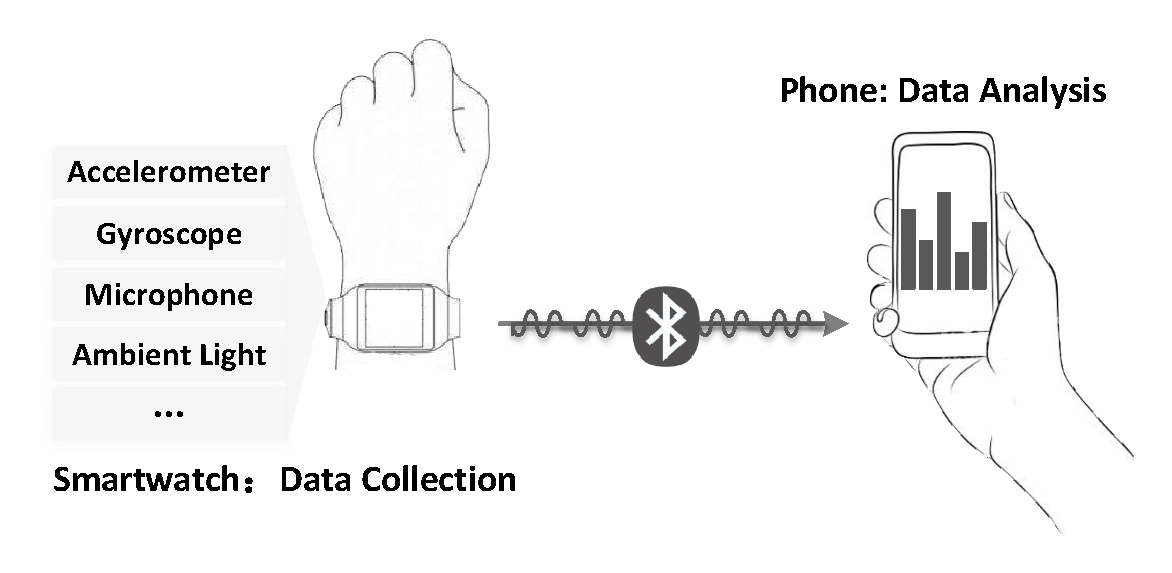
\includegraphics[width=0.5\textwidth]{Figures/datacollect.pdf}
  \caption{Our approach detects a wide range of sleep-related activities and events using a smartwatch.}\label{fig:datacollect}
\end{figure}

This paper presents novel approach to gather a richer set of fine-grained sleep events. Instead of using smartphones and relying on strict,
unrealistic assumptions, we exploit the rich sensor data provided by smartwatches to track a wider range of sleep-related activities. The
advantages of using a smartwatch are that many users are willing to wear the device throughout the night, thus the device can remain
relatively close to the user over the duration of sleep. The smartwatch also allows us to collect a richer set of information. The
collected information can then be used to monitor a wider range of sleep-related events. While there are prior works on sleep monitoring
based on smartwathes \cite{pombo2016ubisleep,shelgikar2016sleep,haescher2015anomaly,borazio2012combining}, these approaches only gather
coarse-grained information and often rely on specialize devices such as pressure mattresses or image acquisition equipment. In this
article, we demonstrate that, for the first time, smartwatches can be used to collect an extensive set of sleep-related events -- many of
which are not presented in prior work. Having a more comprehensive set of sleep-related events and activities will thus enable users to
gain a deeper understanding of their sleep patterns and the causes of poor sleep.

We implement our approach in a prototype system called \systemname. It gathers sleep-related activities by utilizing the commonly available
sensors on smartwatches: the accelerometer, gyroscope, microphone and ambient light sensor, etc. It then uses the tracked information to
infer the user's sleep posture and habits -- thing like changes of body and hand positions, as well as sound events due to e.g. snoring or
coughing.  Collecting these data can help a user to gain a deep understanding of his/her sleeping pattern and quality, and to find ways to
improve sleep. \FIXME{ZW: The introduction is too wordy. It needs to get to the point quicker. I will get back to this later.}

Translating the collected sensor data to these sleeping events is non-trivial due to the changing nature of smartwatches during sleep. To
overcome these challenges, we develop a set of new methods and analysis, specifically targeting portable mobile devices.  The key insight
behinds {\systemname} is that the sleep quality is strongly correlated to the sleep posture, acoustic events and the illumination condition
\cite{shelgikar2016sleep}. By exploiting the unique characteristics of sensory data produced by different sleep activities, we develop a
series of novel algorithms to correlate the sensory data to sleep events. We then design a model to incorporate the detected events to
infer the user's sleep stages and sleep quality. \FIXME{ZW: This one needs to be merged with the previous paragraph.}

 We evaluate our approach through extensive experiments involved ten uses over a period of two weeks. The experimental results
show that {\systemname} is effective and accurate in capturing sleep-related activities, achieving an accuracy of at least 87\% (up to
98\%) across various sleep events. We demonstrate that these fine-grained sleep data enable us to develop an accurate model to correlate
the sleep events to various sleep stages, helping user to better understand their sleep quality. 

The main contribution of this paper is the first smartwatch-based system that can capture a wider range of sleep events with a high
accuracy. We show that, compared with existing mobile-based sleep monitoring solutions, the rich set of fine-grained sleep events given by
our approach can better capture a user's sleep patterns and quality across sleep stages.
